\documentclass[12pt, class=report, crop=false]{standalone}
\usepackage{ba_thesis}

\begin{document}

\chapter{The Interaction Between Electromagnetic Radiation and Matter}%
\label{chap:light-matter-interaction}
Now that the aspects related to the formalism and theory behind the modeling of laser produced electromagnetic waves has been presented, we must naturally turn our attention towards the interaction of those wave pulses with matter. This chapter only deals with the dinamics of particles under the action of electromagnetic fields and the ponderomotive force, since these topics offer great insight and intuition for the physical behaviour of high intensity laser-plasma interaction. The specific phenomena arising from the properties of plasma as a medium are to be presented later.
\section{Electron Dynamics in Electromagnetic Fields}
This section deals with analyzing the motion of a single electron in the fields of a wave. For simplicity, I will only talk about the case of linearly polarized plane waves, since this entire discussion has the purpose of building up intuition and getting a feel for the scale of the relevant quantities. Most of what is to be presented is following the lecture notes of~\cite{karschApplicationsHighIntensity2018}.

The fact that we want to study dynamics and we are using a very simple type of wave means that it is actually more convenient this time around to work with real fields, rather than complex ones. As per usual, the direction of propagation is chosen to be the z-axis such that the fields are

\begin{subequations}
  \begin{align}
    \vb{E} =\vb{e_x} E_0 \cos(kz-\omega t) \\
    \vb{B} =\vb{e_y} B_0 \cos(kz-\omega t)\,.
  \end{align}
\end{subequations}
Just as an exercise, it can be observed that these fields are generated by the following choice for the 4-potential

\begin{equation}
  \label{choice:potentials}
  \begin{cases}
    \phi = 0 \\
    \vb{A} = \vb{e_x} A_0 \sin(kz-\omega t)\,,
  \end{cases}
\end{equation}
where \(A_0 = \frac{E_0}{\omega} = \frac{B_0}{k}\).
\subsection{Classical Treatment}

We start from the classical equation of motion given by Newton's second principle using the Lorentz force

\begin{equation}
  \label{eq:equation-of-motion-electron}
  \dv{\vb{p}}{t} = \dv{(m_e \vb{v_e})}{t} = - e \left( \vb{E} + \vb{v_e}\cp\vb{B} \right)\,,
\end{equation}
with \(m_e\) and \(\vb{v_e}\) the mass and the velocity of the electron, respectively, and \(e\) the elementary charge. Since we have \(B\propto\frac{E}{c}\) and also \(v_e \ll c\) (which is implied in order to have a classical treatment), we can safely remove the second term in the right-hand side of the equation above, remaining with

\begin{equation}
  \dv{\vb{v_e}}{t} = - \frac{e}{m_e} \vb{E} = - \frac{e}{m_e}  E_0 \vb{e_x} \cos(kz-\omega t)\,.
\end{equation}
Simply integrating with initial conditions \(x_0\), \(y_0\), \(z_0\) \(=0\) and \(\vb{v_e(0)} = \vb{0}\) leads to

\begin{subequations}
  \begin{align}
    \vb{v_e} (t) = \frac{e}{\omega m_e} E_0 \vb{e_x} \sin(kz-\omega t) \\
    x (t) = \frac{e}{\omega^2 m_e} E_0 \left[ \cos(kz-\omega t) -1 \right]\,.
  \end{align}
\end{subequations}

It is important now to see when the classical treatment breaks down. Let us impose that

\begin{equation}
  v_e^{max} = c \,,
\end{equation}
such that we have

\begin{equation}
  a_0 \equiv \frac{e E_0}{\omega m_e c} = \frac{e A_0}{m_e c} = 1\,.
\end{equation}
The parameter \(a_0\) is called the normalized or dimensionless vector potential. From its definition it is easy to see that it can only take values between 0 and 1. We can use it to describe the amplitude of the electric field as such

\begin{equation}
  E_0 = a_0 \frac{\omega m_e c}{e}\,.
\end{equation}
It is very convenient in practice to use the wavelength and to extract the rest mass to charge ratio of the electron as follows

\begin{equation}
  E_0 = \frac{a_0}{\lambda} 2\pi \frac{m_e c^2}{e} = \frac{a_0}{\lambda} 2\pi\cdot 511 kV\,.
\end{equation}
The normalized vector field helds also an important significance. One can see that its definition actually boils down to

\begin{equation}
  a_0 = \frac{v_{max}^{classical}}{c}\,,
\end{equation}
so we can use it to find a boundary for the validity of the classical treatment. For simplicity, lets disect the \(a_0 = 1\) case, for which the motion should be completely relativistic, keeping in mind that the classical description stops being reliable well befor that. From the result concerning the Poynting vector of a plane wave~(\ref{def:poynting-plane-wave}), we can find the intensity of the pulse in this limiting case to be

\begin{equation}
  I = c \frac{\varepsilon_0}{2} E_0^2 \propto \frac{a_0^2}{\lambda^2} 10^{18} W \frac{\mu m^2}{cm^2}\;,
\end{equation}
which says that already at intensities of \(10^{18} \frac{W}{cm^2}\) the motion of the electron should be treated completely within the grounds of special relativity.

\subsection{Relativistic Treatment}
In the light of our discussion in the previous subsection, we see that in order to study how electrons interact with high-intensity laser beams (namely, terwatt and petawatt lasers), we should do all our calculations relativistically. The equation of motion remains the same, but the relativistic momentum is \(\vb{p} = \gamma m_e \vb{v_e}\), where \(\gamma\) is the usual Lorentz factor. By taking the scalar product of~\cref{eq:equation-of-motion-electron} with \(\vb{p}\) we get

\begin{equation}
  \frac{1}{2} \dv{\vb{p}^2}{t} = - e \vb{p}\vdot\vb{E}\,,
\end{equation}
where we used the fact that \(\vb{p}\vdot\left(\vb{v_e}\cp\vb{B}\right)\), since \(\vb{p}\) is proportional to \(\vb{v_e}\). Now, it is useful to write the Lorenz factor in terms of momentum like this

\begin{equation*}
  \gamma = \frac{1}{\sqrt{1 - \frac{\vb{v}^2}{c^2}}} \Rightarrow
  \frac{1}{\gamma^2} = 1 - \frac{\vb{v}^2}{c^2} = 1 - \frac{1}{\gamma^2} \frac{\vb{p}^2}{m_e^2 c^2} \Rightarrow \gamma = \sqrt{1+\left(\frac{\vb{p}}{m_e c}\right)^2} \,.
\end{equation*}
Now we can expect to find a \(\dv{\vb{p}^2}{t}\) by taking the derivative of \(\gamma\) with respect to time

\begin{equation*}
  \dv{\gamma}{t} = \dv{t} \sqrt{1+\left(\frac{\vb{p}}{m_e c}\right)^2} = \frac{1}{\sqrt{1+\left(\frac{\vb{p}}{m_e c}\right)^2} } \frac{1}{m_e^2 c^2} \frac{1}{2} \dv{\vb{p}^2}{t} = \frac{1}{\gamma m_e^2 c^2}\frac{1}{2} \dv{\vb{p}^2}{t} \Rightarrow
\end{equation*}

\begin{equation*}
  \Rightarrow m_e c^2 \dv{\gamma}{t} = - e \frac{\vb{p}}{\gamma m_e} \vdot \vb{E} = -e \vb{v_e}\vdot\vb{E}\,.
\end{equation*}
Remembering that the kinetic energy in special relativity is obtained as \(K = (\gamma - 1) m_e c^2\), we can reach an equation for it

\begin{equation}
  \dv{K}{t} = -e \vb{v_e}\vdot\vb{E}\,.
\end{equation}
This equation can also be rewritten as

\begin{equation}
  \label{eq:gamma-vx}
  \dv{\gamma}{t} = -\frac{e E_0}{m_e c} \frac{\vb{v_e}\vdot\vb{e_x}}{c} \cos(kz-\omega t) = - a_0 \omega \frac{v_x}{c} \cos(kz-\omega t)\,.
\end{equation}
In order to procees, we should also take a better look at the equation of motion as it is

\begin{equation*}
  \dv{t} (\frac{\vb{p}}{m_e c}) = - \frac{e}{m_e c} \left[E_0 \vb{e_x} + B_0 \vb{v}\cp\vb{e_y}\right]\cos(kz-\omega t) =
\end{equation*}

\begin{equation*}
  = - \frac{e E_0}{m_e c} \left[\vb{e_x} + \frac{\vb{v}}{c}\cp\vb{e_y} \right]\cos(kz-\omega t) =
\end{equation*}

\begin{equation*}
  = -a_0 \omega \left[ \left(1 - \frac{v_z}{c} \right)\vb{e_x} + \frac{v_x}{c} \vb{e_z} \right]\cos(kz-\omega t)\,.
\end{equation*}
By defining \(\vb{\tilde{p}} = \frac{\vb{p}}{m_e c}\) to be the normalized momentum, we can write the equations for its components as follows

\begin{subequations}
  \begin{flalign}
    \label{eq:momentum-x}
    \dv{\tilde{p_x}}{t} = -a_0 \omega \left(1 - \frac{v_z}{c} \right) \cos(kz-\omega t) \\
    \dv{\tilde{p_y}}{t} = 0 \\
    \label{eq:momentum-z}
    \dv{\tilde{p_z}}{t} = -a_0 \omega \frac{v_x}{c} \cos(kz-\omega t)\,.
  \end{flalign}
\end{subequations}
The \(y\) is trivial, and since we took the initial velocity to be zero, the \(y\)-velocity will be zero at all times.

From~\cref{eq:gamma-vx,eq:momentum-z} we have the following developement

\begin{equation}
  \dv{(\tilde{p_z}-\gamma)}{t} = 0 \Leftrightarrow \tilde{p_z}-\gamma = C \,.
\end{equation}
Again, making use of our choice of initial conditions, which translate here as \(\gamma (0) = 1\) and \(\tilde{p_z} (0)= 0\), we obtain \(C\) to be -1.

To summarize so far, we already know that

\begin{subequations}
  \begin{align}
    \tilde{p_y} = 0\\
    \label{sol:pz2}
    \tilde{p_z} = \gamma - 1\,.
  \end{align}
\end{subequations}
By squaring up the very last equation, yet another useful relation can be derived

\begin{equation*}
  \gamma = 1 + \tilde{p_z} = \sqrt{1+\vb{\tilde{p}}} \Rightarrow 1+2\tilde{p_z}+ \tilde{p_z}^2 = 1+\tilde{p_x}+\tilde{p_y}+\tilde{p_z}
\end{equation*}

\begin{equation}
  \label{sol:pz}
  \tilde{p_z} =  \frac{1}{2} \tilde{p_x}^2\,.
\end{equation}
Since \(p_z\) is the normalized momentum along the propagation direction of the wave, we can see that for \(\tilde{p_z} =  \frac{1}{2} \tilde{p_x}^2 \ll 1\) (classical regime) the transversal momentum is more important, while for \(\tilde{p_z} =  \frac{1}{2} \tilde{p_x}^2 \gg 1\) (highly relativistic regime) the longitudinal momentum is more important.

Now we would like to find \(p_x\). There is actually a more efficient way to do so than solving~\cref{eq:momentum-x,eq:momentum-z} together. But for that we shall make use of the electromagnetic potential~(\ref{choice:potentials}). We also need the relations that define the fields from the potential, as detailed in section~(\ref{ch-ref-1}). With this in mind, we return to the equation of motion

\begin{equation}
  \dv{\vb{p}}{t} = - e \left( \vb{E} + \vb{v_e}\cp\vb{B} \right) = -e \left( -\partial_t \vb{A} + \vb{v_e}\cp(\curl{\vb{A}}) \right)\,.
\end{equation}
We make use of the vector identity

\begin{equation}
  \label{id:vp-of-curl}
  \vb{v}\cp(\curl{\vb{u}}) = \grad{(\vb{v}\vdot\vb{u})} - (\vb{v}\vdot \grad) \vb{u}\,,
\end{equation}
and the total derivative of \(A\) with respect to time

\begin{equation}
  \dv{\vb{A}}{t} =
  \partial_t \vb{A} + \partial_{x_i} A^{x_i} \partial_t x_i =
  \pdv{\vb{A}}{t} + (\vb{v_e}\vdot \grad) \vb{A}\,.
\end{equation}
Thus,

\begin{equation}
  \dv{\vb{p}}{t} = - e \left[ -\dv{\vb{A}}{t} + (\vb{v_e}\vdot \grad) \vb{A} + \grad{(\vb{v_e}\vdot\vb{A})} - (\vb{v_e}\vdot \grad) \vb{A} \right] = - e \left[ -\dv{\vb{A}}{t} + \grad{(\vb{v_e}\vdot\vb{A})} \right]\,.
\end{equation}
Since

\begin{equation*}
  \dv{\vb{A}}{t} = - \vb{e_x} \omega A_0 \cos(kz-\omega t)
\end{equation*}

\begin{equation*}
  \grad{(\vb{v_e}\vdot\vb{A})} = \vb{e_z} k v_x A_0 \cos(kz-\omega t)\,,
\end{equation*}
we can extract the \(p_x\) equation

\begin{equation}
  \dv{p_x}{t} = - e \omega A_0 \cos(kz-\omega t) = e \dv{A}{t}\,,
\end{equation}
which gives

\begin{equation}
  p_x = eA + C'\,.
\end{equation}
With the initial conditions this becomes

\begin{equation}
  \label{sol:px}
  p_x = e A = e A_0 \sin(kz-\omega t)\,.
\end{equation}

Bringing together~\cref{sol:px,sol:pz,sol:pz2}, using the normalized vector potential \(a = \frac{e A_0}{m_e c} \sin(kz-\omega t)\)

\begin{equation}
  K = (\gamma -1)m_e c^2 =\frac{a^2}{2}m_e c^2 \Rightarrow \gamma = 1 + \frac{a^2}{2}\,.
\end{equation}

With this, all the puzzle pieces are in place, so we can collect the following results concerning the motion of the electron

\begin{subequations}
  \begin{align}
    \gamma = 1 + \frac{a^2}{2}\\
    \tilde{p_x} = a\\
    \tilde{p_y} = 0\\
    \tilde{p_z} = \frac{a^2}{2}\,.
  \end{align}
\end{subequations}
It is more convenient, and general, to work with the derivative with respect to \(\tau = t - \frac{z(t)}{c}\), which is to choose the convenient reference frame of the wave to simplify the computations. This derivative is developed as such

\begin{equation}
  \dv{t} = \dv{\tau}{t} \dv{\tau} = \left( 1 - \frac{1}{c} \dv{z}{t} \right) \dv{\tau} = \left( 1 - \frac{a^2}{2}  \right) \dv{\tau} = \frac{1}{\gamma} \dv{\tau}\,.
\end{equation}
We can also write the phase of \(a\) in terms of this time

\begin{equation}
  kz-\omega  t= kz -\omega\tau - \frac{\omega}{c} z = - \omega \tau\,.
\end{equation}
A simple substitution gives the equations for the coordinates

\begin{subequations}
  \begin{align}
    \dv{x}{\tau} = c a\\
    \dv{y}{\tau} = 0\\
    \dv{z}{\tau} = c \frac{a^2}{2}\,,
  \end{align}
\end{subequations}
which have the solutions (of course using the initial conditions we chose at the begining)

\begin{subequations}
  \begin{align}
    x(\tau) = \frac{ca_0}{\omega} \left[\cos(\omega \tau) - 1 \right] \\
    y(\tau) = 0\\
    z(\tau) = \frac{ca_0^2}{4} \left[\tau - \frac{1}{2\omega} \sin(2\omega \tau)\right]\,.
  \end{align}
\end{subequations}

These results show us that the motion in the transversal plane is the same as in the classical motion. However, the motion on the propagation direction is more complex, being a superposition of an oscillation and a drift motion. The drift velocity \(v_{drift} = \expval{v_z} = \expval{\frac{z}{t}}\) can be computed fairly easy

\begin{equation*}
  z_{drift} = \frac{ca_0^2}{4} \tau = \frac{ca_0^2}{4} \left( t - \frac{z}{c} \right) = \frac{ca_0^2}{4} t - \frac{a_0^2}{4} z_{drift}
\end{equation*}

\begin{equation*}
  z_{drift} = \frac{ca_0^2}{4} \frac{t}{1+\frac{a_0^2}{4}} = \frac{ca_0^2}{4+a_0^2} t
\end{equation*}

\begin{equation}
  v_{drift} = \frac{ca_0^2}{4+a_0^2}\,.
\end{equation}

\begin{figure}[h]
  \centering
  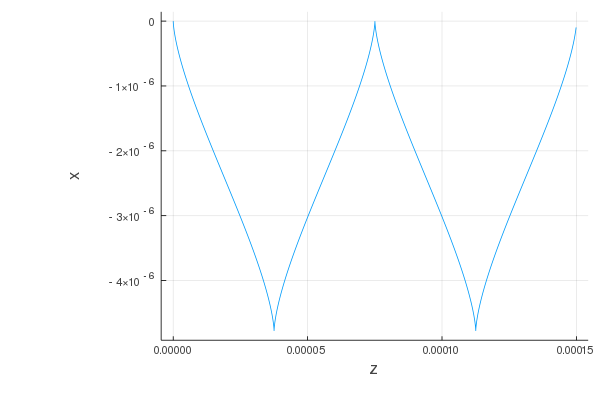
\includegraphics[width=0.65\textwidth]{relativistic_electron_cont_pulse}%
  \caption{The motion in the laboratory frame over two periods of the pulse for some practical parameters: \(a_0 = 20\) and \(\nu=\frac{\omega}{2\pi} = 400\) THz}\label{fig:electron-motion-cont}%
\end{figure}

In finite length pulses, a certain phenomenon occurs. In order to obtain a finite plane wave pulse, we simply add a Gaussian envelope

\begin{equation}
  a(\tau) = a_0 \exp(-\left(\frac{\tau}{\tau_0}\right)^2) \sin(\omega \tau)\,.
\end{equation}
Under the fields given by this potential, the electron starts moving, but it stops when the wave passes it. Thus, although the electron is moved forward, the net energy gain in its interaction with the field is zero. The theoretical calculations that prove this are quite lengthy, so, in order to visualize this effect, I offer a numerical solution of this motion solved using an explicit Euler method in~\cref{fig:electron-motion-pulse}. The step-size used was small enough that the instability of the method is not relevant. The Julia code used is available in the Appendix at the end of the thesis. We can see that the trajectory of the electron converges to a point after a time longer than the pulse duration.

\begin{figure}[h]
  \centering
  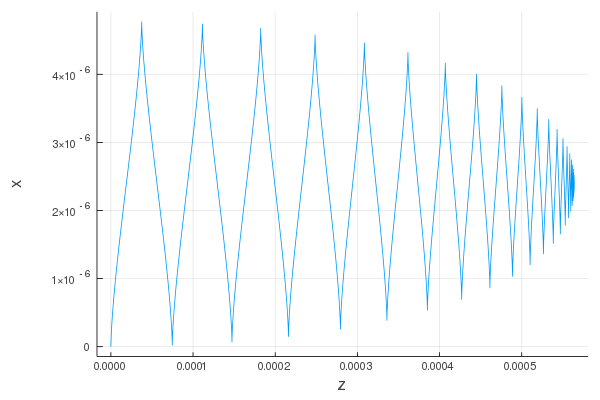
\includegraphics[width=0.7\textwidth]{relativistic_electron_short_pulse}%
  \caption{The motion in the laboratory frame over a long time compared to the pulse duration \(\tau_0\). The parameters used were: \(a_0 = 20\), \(\tau_0 = 30\) fs and \(\nu=\frac{\omega}{2\pi} = 400\) THz}\label{fig:electron-motion-pulse}%
\end{figure}

While a rigurous and complete discussion on dinamics of electrons in wave fields can take an entire book, I will offer here the Lawson-Woodward theorem, which analyzes the posibility for an electron to be accelerated by an electromagnetic wave.

\subsubsection{Theorem(Lawson-Woodward)}
A reletivistic electron does not gain energy from an electromagnetic wave if
\begin{itemize}
  \item if the interaction takes place in vacuum, in the abence of any walls or any other particles;
  \item if the electron is in the highly relativistic regime during the entire acceleration process;
  \item if there are no static electromagnetic fields;
  \item if the interaction region is infinitely large;
  \item if the ponderomotive force can be neglected.
\end{itemize}
If at least one of these conditions are violated, acceleration can happen.
\newline

In laser-plasma interaction in particular, all the conditions of this theorem are not valid, which is why the possibility of developing a plasma based, laser powered accelerator is appealing. More on the prospects of this technology will be presented in the next sections.

\section{The Ponderomotive Force}

In this section we will delve into the most relevant physical phenomenon for our studies, namely the ponderomotive force. Intuitively, if we have a focused laser beam, its field will strongly vary in the transverse direction. For an electron that is initially found on the axis of the pulse, the deflection is stronger than the restoring force. Because of this, the electron will be completely removed from the focal region after a couple of oscillations and will retain a non-zero kinetic energy. This effect is called ponderomotive scattering. Some results from simulations of electron movement in various laser beam profiles are presented later in~\cref{sec:ponderomotive-graphs}. In these simulations we solved numerically the equations of motion for the electron, but in this section we will do some approximated computations to get a better understanding of the physics that generate this effect.

\subsection{Classical Derivation}

We already solved the motion of the electron in a plane wave, but for our current purpose, we will need a more general expression for the field. Namely, we would like to have a periodic dependence on time and a spatial dependence of the amplitude

\begin{equation}
  \vb{E} = \vb{E_0}(\vb{r}) \cos(\omega t)\,.
\end{equation}
Note that the plane wave field is just a particular case of this ansaz, but now the equation of motion~(\ref{eq:equation-of-motion-electron}) is valid only locally, at the electron position \(\vb{r_0}\). Let us approxiamates the field around \(\vb{r_0}\) by Taylor expansion

\begin{equation}
  \vb{E_0}(\vb{r}) = \left[\vb{E_0}(\vb{r})\right]_{\vb{r}=\vb{r_0}} + \left[(\delta \vb{r}\vdot\grad)\vb{E_0}(\vb{r})\right] _{\vb{r}=\vb{r_0}} + \mathcal{O}(\delta\vb{r}^2)\,.
\end{equation}
From the Maxwell equation \(\partial_t \vb{B} = - \curl{\vb{E}}\), by integration over time, we can also find the magnetic field

\begin{equation}
  \vb{B}(\vb{r}) =\frac{1}{c}\left[\vb{e_z} \cp \vb{E_0}(\vb{r})\right]_{\vb{r}=\vb{r_0}} \cos(\omega t) - \frac{1}{\omega} \left[\curl{\vb{E_0}(\vb{r})}\right]_{\vb{r}=\vb{r_0}} \sin(\omega t)\,.
\end{equation}
We can now write the equation of motion in first order and in second order, respectively

\begin{subequations}
  \begin{align}
    \label{eq:first-order}
    m_e \dv{\vb{v}^{(0)}}{t} = - e \left[\vb{E_0}(\vb{r_0}) \cos(\omega t) + \frac{\vb{v}^{(0)}}{c}\cp \left(\vb{e_z} \cp \vb{E_0}(\vb{r_0}) \right) \cos(\omega t)\right] \approx - e \vb{E_0}(\vb{r_0}) \cos(\omega t)\\
    \label{eq:second-order}
    m_e\dv{\vb{v}^{(1)}}{t} = - e \left[ (\delta\vb{r}\vdot\grad) \vb{E_0}(\vb{r})\right]_{\vb{r}=\vb{r_0}} \cos(\omega t) + e \frac{1}{\omega} \vb{v}^{(0)}\cp \left[\curl{\vb{E_0}(\vb{r})}\right]_{\vb{r}=\vb{r_0}} \sin(\omega t) \,,
  \end{align}
\end{subequations}
where \(\dv{(\delta \vb{r})}{t} = \vb{v}^{(0)}\) and we have used the fact that \(v^{(0)}\ll c\).Equation~(\ref{eq:first-order}) is solved by direct integration

\begin{subequations}
  \begin{align}
    \vb{v}^{(0)} = - \frac{e}{m_e \omega} \vb{E_0}(\vb{r_0}) \sin(\omega t)\\
    \delta \vb{r} = \frac{e}{m_e \omega^2} \vb{E_0}(\vb{r_0}) \cos(\omega t)\,.
  \end{align}
\end{subequations}
These are pretty much the results from the plane wave, that is the oscillatory motion induced by the wave on the electron. The second order equation describes an additional effectthat arises. Replacing the above solutions in~\cref{eq:second-order} leads to

\begin{equation}
    m_e\dv{\vb{v}^{(1)}}{t} = - \frac{e^2}{m_e \omega^2} \left[ (\vb{E_0}\vdot\grad)\vb{E_0}\cos[2](\omega t) + \vb{E_0}\cp\left(\curl{\vb{E_0}}\right)\sin[2](\omega t) \right]_{\vb{r}=\vb{r_0}}\,.
\end{equation}
So far this discussion followed the microscopic motion. We are intrested in average effects, so we should find the time average of the expression obtained. Keeping in mind that both the averages of sine squared and cosine squared over one period are one half, we can deduce that

\begin{equation}
  \expval{m_e\dv{\vb{v}^{(1)}}{t}}_T =  - \frac{e^2}{2 m_e \omega^2} \left[ (\vb{E_0}\vdot\grad)\vb{E_0} + \vb{E_0}\cp\left(\curl{\vb{E_0}}\right)\right]_{\vb{r}=\vb{r_0}}\,,
\end{equation}
where \(T=\frac{2\pi}{\omega}\).
We aplly now the vector identity~(\ref{id:vp-of-curl}) and the fact that \(\grad{\vb{v}^2} = 2\vb{v}(\div{\vb{v}})\) to reach the final result

\begin{equation}
  \expval{m_e\dv{\vb{v}^{(1)}}{t}}_T = - \frac{e^2}{4 m_e \omega^2} \grad{\vb{E_0}^2} = \vb{F_{pond}}\,,
\end{equation}
which gives the expression of the ponderomotive force \(\vb{F_{pond}}\).

\subsection{Relativistic Ponderomotive Force}

We already saw that for high intensity lasers the classical treatment is insufficient. In the case of the ponderomotive force a relativistic derivation leads to the same dependence on the field. More precisely, the ponderomotive force is directly proportional to the gradient of the squared electric field. Nonetheless, I will try to present in this section a rigurous relativistic treatment based on the discussion in the 5th chapter of~\cite{mulserHighPowerLasermatter2010}.

We will start with the Lagrangian for an electron in an arbitrary 4-vector potential \((\phi,\vb{A})\)

\begin{equation}
  \label{eq:lagrangian-0}
  L(\vb{x},\vb{v},t) = -\frac{m_e c^2}{\gamma} - e\vb{v}\vdot\vb{A} + e \phi\,.
\end{equation}
Since our system has an oscillation part given by the periodic time dependence of the 4-vector potential of the driving electromagnetic wave, we can change to action-angle variables \(S=S(\vb{x},t)\) and \(\eta = \eta (\vb{x},t)\), which are Lorentz invariant, so the motion will be governed by Hamilton's principle

\begin{equation}
  \label{eq:new-action}
  \delta S = \delta \int_{\eta_i}^{\eta_f} \dd{\eta} L(\vb{x}(\eta),\vb{v}(\eta),t(\eta)) \dv{t}{\eta}\,.
\end{equation}
This change of variables introduces a new Lagrangian (a ``Lagrangian angular density'' if you want)

\begin{equation}
  \label{eq:new-lagrangian}
  \mathcal{L} (\eta) = \frac{L(\eta)}{\dv{\eta}{t}}\,.
\end{equation}
With all these things set up and choosing \(\eta\) to be normalized to \(2\pi\), we introduce the cycle averaged Lagrangian

\begin{equation}
  \label{eq:cycle-avg-lagrangian}
  \mathcal{L}_0 (\eta) = \frac{1}{2\pi} \int_\eta^{\eta+2\pi} \dd{\eta'} \mathcal{L} (\eta')\,.
\end{equation}
We denote by \(N = \frac{n_f-n_1}{2\pi}\) to be the number of cycles over which \(\mathcal{L}_0\) undergoes a significant change. We are interested now to see how \(N\) imposes a boundary on the action of \(\mathcal{L}_0\). From~\cref{eq:new-action,eq:new-lagrangian} we see that

\begin{equation*}
  \delta \int_{\eta_i}^{\eta_f} \dd{\eta} \mathcal{L} = 0\,,
\end{equation*}
which is useful in order to do the following mathematical arguments

\begin{equation*}
  \abs{\delta \int_{\eta_i}^{\eta_f} \dd{\eta} \mathcal{L}_0} = \abs{\delta \int_{\eta_i}^{\eta_f} \dd{\eta} (\mathcal{L}_0 - \mathcal{L})} = \abs{\int_{\eta_i}^{\eta_f} \dd{\eta} \delta (\mathcal{L}_0 - \mathcal{L})} =
\end{equation*}

\begin{equation*}
  = \abs{\int_{\eta_i}^{\eta_f} \dd{\eta} \left[\mathcal{L}_0 (\eta+\delta\eta) - \mathcal{L}(\eta+\delta\eta) \right] - \int_{\eta_i}^{\eta_f} \dd{\eta} \left[\mathcal{L}_0 (\eta) - \mathcal{L}(\eta) \right]} \leq
\end{equation*}

\begin{equation*}
  \leq \sum_{n=1}^{N} \abs{\int_{\eta_n}^{\eta_n + 2\pi} \dd{\eta} \left[\mathcal{L}_0 (\eta+\delta\eta) - \mathcal{L}(\eta+\delta\eta) \right] - \int_{\eta_n}^{\eta_n + 2\pi} \dd{\eta} \left[\mathcal{L}_0 (\eta) - \mathcal{L}(\eta) \right]}\,,
\end{equation*}
where we discretized the angle variable as \(\eta_n = \eta_i +2\pi n\), \(n \in \mathbb{N}^*\) and used the triangle inequality for the modulus. We will now replace \(\mathcal{L}\) from~\cref{eq:cycle-avg-lagrangian} and continue our endeavours

\begin{equation*}
  \abs{\delta \int_{\eta_i}^{\eta_f} \dd{\eta} \mathcal{L}_0} \leq \sum_{n=1}^{N} \abs{\int_{\eta_n}^{\eta_n + 2\pi} \dd{\eta} \mathcal{L}_0 (\eta+\delta\eta) - 2 \pi \mathcal{L}_0 (\eta_n +\delta\eta_n) - \int_{\eta_n}^{\eta_n + 2\pi} \dd{\eta} \mathcal{L}_0 (\eta) - 2\pi \mathcal{L}_0 (\eta_n)} =
\end{equation*}

\begin{equation*}
  = \sum_{n=1}^{N} \abs{\int_{\eta_n}^{\eta_n + 2\pi} \dd{\eta} \left[ \mathcal{L}_0 (\eta+\delta\eta) - \mathcal{L}_0 (\eta)\right] - 2\pi \left[ \mathcal{L}_0 (\eta_n+\delta\eta_n) - \mathcal{L}_0 (\eta_n)\right]} \approx
\end{equation*}

\begin{equation*}
  \approx \sum_{n=1}^{N} \abs{\int_{\eta_n}^{\eta_n + 2\pi} \dd{\eta} \pdv{\mathcal{L}_0 (\eta)}{\eta} \delta \eta -2\pi \pdv{\mathcal{L}_0 (\eta_n)}{\eta_n} \delta \eta_n}\,,
\end{equation*}
where we kept only the first terms in \(\delta \eta\) and \(\delta \eta_n\). Now, it is time to use the mean value theorem to evaluate the integral

\begin{equation*}
  \int_{\eta_n}^{\eta_n + 2\pi} \dd{\eta} \pdv{\mathcal{L}_0 (\eta)}{\eta} \delta \eta = 2 \pi \pdv{\mathcal{L}_0 (\eta_n^c)}{\eta_n^c} \delta \eta_n^c\,,
\end{equation*}
with \(\eta_n^c \in (\eta_n, \eta_n +2\pi)\), to obtain

\begin{equation*}
  \abs{\delta \int_{\eta_i}^{\eta_f} \dd{\eta} \mathcal{L}_0} \leq 2\pi \sum_{n=1}^{N} \abs{\pdv{\mathcal{L}_0 (\eta_n^c)}{\eta_n^c} \delta \eta_n^c - \pdv{\mathcal{L}_0 (\eta_n)}{\eta_n} \delta \eta_n} = 2\pi \sum_{n=1}^{N} \abs{\left[\pdv{\mathcal{L}_0 (\eta)}{\eta} \delta \eta\right]_{\eta=\eta_n^c} - \left[\pdv{\mathcal{L}_0 (\eta)}{\eta} \delta \eta\right]_{\eta=\eta_n}}\,.
\end{equation*}
We can also use a first order expansion to simplify the quantity in the modulus

\begin{equation*}
  \abs{\left[\pdv{\mathcal{L}_0 (\eta)}{\eta} \delta \eta\right]_{\eta=\eta_n^c} - \left[\pdv{\mathcal{L}_0 (\eta)}{\eta} \delta \eta\right]_{\eta=\eta_n}} =
\end{equation*}

\begin{equation*}
  = \abs{\left[\pdv{\mathcal{L}_0 (\eta)}{\eta} \delta \eta\right]_{\eta=\eta_n^c} - \left[\pdv{\mathcal{L}_0 (\eta)}{\eta} \delta \eta\right]_{\eta=\eta_n^c} - \left[\pdv[2]{\mathcal{L}_0 (\eta)}{\eta} \delta \eta\right]_{\eta = \eta_n^c} (\eta_n - \eta_n^c)} =
\end{equation*}

\begin{equation*}
  = \abs{\left[\pdv[2]{\mathcal{L}_0 (\eta)}{\eta} \delta \eta\right]_{\eta = \eta_n^c}} \abs{\eta_n - \eta_n^c)} \leq
\end{equation*}

\begin{equation*}
  \leq 2\pi \abs{\left[\pdv[2]{\mathcal{L}_0 (\eta)}{\eta} \delta \eta\right]_{\eta = \eta_n^c}}\,,
\end{equation*}
so that in the end we remain with

\begin{equation}
  \label{eq:bound-of-cyc-lag}
  \abs{\delta \int_{\eta_i}^{\eta_f} \dd{\eta} \mathcal{L}_0} \leq (2\pi)^2 \sum_{n=1}^{N} \abs{\left[\pdv[2]{\mathcal{L}_0 (\eta)}{\eta} \right]_{\eta = \eta_n^c}} \abs{\delta \eta_n^c} \leq (2\pi)^2 N max\left\{\abs{\left[\pdv[2]{\mathcal{L}_0 (\eta)}{\eta} \right]_{\eta = \eta_n^c}}\right\} max\left\{\abs{\delta \eta_n^c}\right\}\,.
\end{equation}
We would want now to impose the condition that \(\mathcal{L}_0^{max}\) changes at most by \(\mathcal{L}_0\) over \(N\) cycles, that is

\begin{equation}
  N = \frac{1}{2\pi} \frac{\abs{\mathcal{L}_0^{max}}}{max\left\{\abs{\left[\pdv{\mathcal{L}_0 (\eta)}{\eta} \right]_{\eta = \eta_n^c}}\right\}}\,.
\end{equation}
By imposing a similar constraint on the first derivative

\begin{equation}
  2 \pi \frac{max\left\{\abs{\left[\pdv[2]{\mathcal{L}_0 (\eta)}{\eta} \right]_{\eta = \eta_n^c}}\right\}}{max\left\{\abs{\left[\pdv{\mathcal{L}_0 (\eta)}{\eta} \right]_{\eta = \eta_n^c}}\right\}} \leq \frac{1}{N}\,,
\end{equation}
we obtain that the action of \(\mathcal{L}_0\) is bounted by a function \(\mathcal{O}(N^{-1})\)

\begin{equation}
  \label{ineq:final-result}
  \abs{\delta \int_{\eta_i}^{\eta_f} \dd{\eta} \mathcal{L}_0} \leq \frac{\abs{\mathcal{L}_0^{max}}}{N} max\left\{\abs{\delta \eta}\right\}\,.
\end{equation}
Let us observe that for the regular averaged lagrangian defined by \(L_0 = \mathcal{L}_0 \dv{\eta}{t}\) we have

\begin{equation}
  \int_{\eta_i}^{\eta_f} \dd{\eta} \mathcal{L}_0 = \int_{t_i}^{t_f} \dd{t} L_0\,.
\end{equation}
If this would be zero, we would get an Euler-Lagrange set of equations for \(L_0\)

\begin{equation}
  \label{eq:euler-lagrange}
  \dv{t} \left(\pdv{L_0}{\vb{v_0}}\right) - \pdv{L_0}{\vb{x_0}} = 0\,,
\end{equation}
where the coordinates \(\vb{x_0}\) and \(\vb{v_0}\) correspond to the oscillation center. However, working with the inequality~(\ref{ineq:final-result}) we would obtain an extra term in the right-hand side of~\cref{eq:euler-lagrange} whose absolute value does not exceed

\begin{equation*}
  \frac{\abs{\mathcal{L}_0^{max}}}{N^2} max\left\{\abs{\delta \eta}\right\}\,.
\end{equation*}
If the Lagrangian \(\mathcal{L}_0\) doesn't depend on time, energy is conserved on average in time and the right-hand side of~\cref{eq:euler-lagrange} is adiabatically zero. For \(N\rightarrow\infty\) it is exactly zero. This extra term is the generalized force associated to the ponderomotive force.

The relativistic Hamiltonian obtained from~\cref{eq:lagrangian-0} by the definition \(H(\vb{x},\vb{p},t)=\vb{p}\vb{v}-L(H(\vb{x},\vb{v},t)\) is

\begin{equation}
  H = \sqrt{m^2 c^4 + c^2(\vb{p}+e\vb{A})^2} - e\phi\,,
\end{equation}
with the canonical momentum defined as

\begin{equation}
  \vb{p} = \pdv{L}{\vb{v}} = \gamma m \vb{v} - e\vb{A}\,.
\end{equation}
By defining the effective mass as

\begin{equation}
  m_{eff} = \frac{\gamma_0 \mathcal{L}_0 \dv{\eta}{t}}{c^2} = \frac{\gamma_0 L_0}{c^2}\,,
\end{equation}
we obtain that the Lagrangian and Hamiltonian in an arbitrary reference system in which the oscillation center moves with velocity \(\vb{v_0}\) are those of a free particle with an effective mass that depends on space-time

\begin{subequations}
  \begin{align}
    L_0 (\vb{x_0},\vb{v_0}, t) = - \frac{m_{eff} c^2}{\gamma_0}\\
    H_0 (\vb{x_0},\vb{p_0}, t) = \gamma_0 m_{eff} c^2\,,
  \end{align}
\end{subequations}
with \(\gamma_0 = \sqrt{1-\frac{\vb{v_0}^2}{c^2}}\) and \(\vb{p_0} = \gamma_0 m_{eff} \vb{v_0}\). In the oscillation center system, the ponderomotive force is defined as

\begin{equation}
  \vb{f_p} \equiv \pdv{L_0}{\vb{x_0}} = -c^2 \grad{m_{eff}}\,.
\end{equation}
For a strong monochromatic electromagnetic wave the effective mass is

\begin{equation}
  m_{eff} = m_e \sqrt{1 + \frac{4}{m_e c^2} \vb{A}^2}\,.
\end{equation}
With this, the classical dependence obtained in the previous subsection still holds

\begin{equation}
  \vb{F_p} \propto \grad{\vb{E}^2}\,.
\end{equation}

% \section{Simulations for the Visualization of the Ponderomotive Force}
% \label{sec:ponderomotive-graphs}

\end{document}
